\chapter[Nutrition, epigenetics, and cancer: an epidemiological perspective]{Nutrition, epigenetics, and cancer: an \\ epidemiological perspective}
\chaptermark{Nutrition, epigenetics, and cancer}
\label{chap2_Nutritionepigeneticscancer: an epidemiologicalperspective}

\AddEverypageHook{%
	\ifthenelse{\equal{\Chaptername}{Nutrition, epigenetics, and cancer}}{
		\ifthenelse{\isodd{\thepage}}%
		{\TileWallPaper{17.4cm}{24.4cm}{thumbCh2.pdf}}%
		{\ClearWallPaper}
	} {\ClearWallPaper}
} 

\quad\\ 
 
\noindent 
Audrey Y. Jung\\ 
Ellen Kampman\\ 
 
\quad\\ 
 
\quad\\ 
 
\quad\\ 
 
\quad\\ 
 
\noindent \emph{Nutrition in Epigenetics (eds M.D. Niculescu and P. Haggarty), Wiley-Blackwell, Oxford, UK (2011). doi: 10.1002/9780470959824.ch20} 
 
\newpage 
 
\noindent Cancer is a multistep process caused by changes in normal cellular mechanisms such as DNA repair, cell cycle, apoptosis, differentiation, proliferation, hormonal regulation, inflammation and immunity, carcinogen metabolism. Errors in any of these functions may lead to altered DNA structure and integrity, apoptosis inhibition, and angiogenesis and/or biologically active chemical induction. Mutations and/or deletions in DNA and aberrant gene expression have also been observed. A common observation in human breast cancers and many other tumour types is epigenetic change consisting of altered methylation of DNA \cite{c21,c22,c23,c24,c25} and the histones associated with DNA \cite{c26,c27,c28}. These changes occur early in the development of cancer and are observed even in low-grade cancers \cite{c29}, with the pattern of methylation correlating with cancer stage \cite{c210}.

\noindent Diet and other environmental exposure such as smoking, physical activity, and overweight may influence carcinogenesis through one or more of the mechanisms depicted in Figure \ref{figure2_1}, and there is ample evidence to support this. Butyrate produced by colonic bacteria, diallyl disulfide in garlic and other \emph{Allium} vegetables, and sulforaphane found in cruciferous vegetables have all been shown to inhibit type I and II HDACs in laboratory studies, thereby helping to maintain DNA stability \cite{c211}. Long-chain \emph{n}-3 polyunsaturated fatty acids (PUFAs) found in fish oils, vitamin D, and retinoic acid have been shown to promote cell differentiation, and, in tumour cells, to limit cell proliferation, and increase apoptosis \cite{c212,c213,c214}. Folate and other methyl donors such as methionine help regulate DNA synthesis and modulate epigenetic mechanisms in DNA \cite{c214}.

\begin{figure} 
\begin{tikzpicture}[ ] 
%Declaration of styles 
\tikzstyle{box} = [rectangle, draw,  rounded corners, minimum width=3.8cm, minimum height=1cm, text centered, draw=black, text width = 3.8cm] %style for the boxes 
\tikzstyle{arr} = [double arrow, draw=black, fill=white] %Style for the arrow 
\tikzstyle{arrs} = [single arrow, draw=black, fill=white] %Style for the arrow 
\tikzstyle{oval} = [ellipse, draw=black, fill=white, minimum height = 3.3cm, text width = 2.3cm, text centered,] 
 
%Nodes, the elements of the graphic 
\node [box] at (0,2.8) {\footnotesize{Epigenetics}};

\node [box] at (-4.2,1.4) {\footnotesize{Carcinogen metabolism}};
\node [box] at (4.2,1.4) { \footnotesize{Inflammation and immunity}};

\node [box] at (-4.5,0) {\footnotesize{Apoptosis}};
\node [box] at (4.5,0) {\footnotesize{Hormonal regulation}};

\node [box] at (-4.2,-1.4) {\footnotesize{Differentiation}};
\node [box] at (4.2,-1.4) {\footnotesize{Proliferation}};

\node [box] at (-2.6,-2.8) {\footnotesize{DNA repair}};
\node [box] at (2.6,-2.8) {\footnotesize{Cell cycle}};

\node [arr, minimum height = 5.4cm, rotate=0] at (0,0) {\quad l\quad};
\node [arr, minimum height = 5.4cm, rotate=33] at (0,0) {\quad l\quad};
\node [arr, minimum height = 5.4cm, rotate=-33] at (0,0) {\quad l\quad};

\node [arrs, minimum height = 2.7cm, rotate=90] at (0,1) {\quad l\quad};
\node [arrs, minimum height = 3.2cm, rotate=-63] at (0.4,-0.9) {\quad l\quad};
\node [arrs, minimum height = 3.2cm, rotate=-117] at (-0.4,-0.9) {\quad l\quad};

\node [oval] at (0,0) {\centering Diet, other lifestyle factors};
\end{tikzpicture} 
\caption{Diet and other lifestyle factors can interfere with the normal functioning of different essential cellular processes, which may affect cancer progression or prevention. (Adapted from the WCRF 2\textsuperscript{nd} Expert Report \cite{c214})}
\label{figure2_1} 
\end{figure}

\noindent The interplay between nutrition and epigenetics in affecting cancer in humans is a relatively new area of research. DNA methylation is by far the most documented and well-studied epigenetic event in human cancers. While many different aberrant epigenetic modifications have been linked to cancer in animal models, laboratory studies, and human observational studies, so far only DNA methylation has been demonstrated to be influenced by nutrition in neoplastic transformations. An explosion in interest in the field of epigenetics, coupled with results from human studies that demonstrate effects of nutrition on DNA methylation and studies in animal models and human cell lines that highlight the effects of nutrition on epigenetic processes, continues to fuel this relatively young field of research. This chapter focuses on the ways in which nutrition can influence epigenetics in carcinogenesis in humans. Although there are a myriad of nutrition-related lifestyle factors that contribute to cancer development or prevention by affecting epigenetic processes, this chapter focuses only on those nutrients that have been shown to influence epigenetic processes in human cancers. We first summarise the many epigenetic modifications that have been implicated in cancer. Then we discuss the current evidence on the link between nutrition and cancer development and progression, with a focus on epigenetics. Finally, we examine the role of nutrition in epigenetic changes in carcinogenesis considering evidence from observational studies, intervention studies, and randomised, placebo-controlled trials.

\section[]{Epigenetics in cancer} % level 1
\noindent Epigenetic modifications continue to garner attention for their role in carcinogenesis. Many epigenetic modifications are known, and DNA methylation is perhaps the most well studied of these. Global DNA hypomethylation is thought to promote genomic instability and it is often found in solid tumours \cite{c215} and leukocytes of individuals with cancer \cite{c216,c217}. In 1983, Feinberg and Vogelstein pioneered the first study to examine DNA methylation changes in primary human tumour tissues \cite{c215}. Studies of adenocarcinoma of the colon and small cell carcinoma of the lung (as well as a liver metastasis derived from the same cell type as the primary small cell lung carcinoma) have demonstrated significant hypomethylation of the growth hormone, $\gamma$-globin, and $\alpha$-globin genes in the tumour compared with surrounding normal cells from the same patient in four of the five types of cancer. Hypomethylation levels in liver metastasis were even greater than in primary tumour. Global hypomethylation in concert with hypermethylation of specific promoters have been found to occur both independently and in conjunction with each other. When occurring together, global hypomethylation has been proposed as an early step in tumourigenesis, while promoter hypermethylation, which often silences tumour suppressor genes and DNA repair genes, is a later event \cite{c218}. Promoter hypermethylation has also been found in colorectal adenomas that precede colorectal carcinomas \cite{c219}. Promoter methylation is found in cytosine-rich areas, termed CpG islands, in areas associated with promoters of functional genes. These CpG islands are normally unmethylated and this is thought to allow gene expression. On the other hand, CpG sites scattered throughout the genome, largely reflecting methylation at repeat sequences and in satellite regions of the DNA, are typically highly methylated, which is important in conferring genomic stability. The number of methylated cytosines is typically reduced in the genomic DNA of tumours compared with normal tissue \cite{c220} and this is associated with shorter survival in colon cancer patients \cite{c221}. DNA methylation patterns change with age, with increases in global hypomethylation and gene-specific hypermethylation as age progresses \cite{c222,c223}.

\noindent Other epigenetic processes such as histone modification have also been implicated in carcinogenesis. Nucleosomes, composed of a fragment of DNA (146 bp) wrapped around a histone octomer, are the fundamental repeating units of chromatin. Histones undergo a myriad of posttranslational alterations including acetylation, which allows the chromatin to unfold and facilitates gene expression \cite{c224}. Aberrant HDAC expression has been found in tumours. Increased HDAC expression has been discovered in gastric cancer, esophageal squamous cell carcinoma, and hormone-refractory prostate cancer \cite{c225,c226}.

\noindent While it is clear that epigenetic alterations influence cancer development, the question of how and why these alterations occur and whether nutritional factors may influence these changes still remain unanswered.
%\vspace{-0.15cm}
\section[]{Nutrition and cancer} % level 1 
\noindent According to the recent World Cancer Research Fund/American Institute of Cancer Research (WCRF/AICR) Second Expert Report, a healthy diet and weight and physical activity can reduce the risk of about a third of all cancers. The WCRF/AICR Report provides evidence from systematic reviews for the protective effects of vegetables and fruits, low body fatness (as measured by body mass index (BMI)), and physical activity on almost all frequently occurring cancers in high-income countries. The WCRF/AICR Panel recommendations were to eat foods mostly of plant origin, to be within the range of normal body weight, and to make physical activity a part of daily life. The Panel also recommended limiting alcohol intake, as there was suggestive evidence that alcohol may increase risk of some cancers \cite{c214}. Here we discuss the evidence in relation to particular nutrients that are thought to influence epigenetic processes.

\subsection{Folate and other B vitamins in cancer} % level 2
\noindent Foods such as green leafy vegetables contain natural folate, while folic acid is the synthetic form of folate and can be found in supplements and fortified foods such as breakfast cereals. Folate has been extensively studied in colorectal cancer (CRC), but results have been inconsistent and inconclusive. Whether folate is protective against or encourages CRC development still needs to be determined \cite{c227}. Although data from cohort studies do show an inverse dose--response relationship, this relationship is not always consistent \cite{c214}. Impairment of these pathways by folate or because of other B vitamin deficiencies may contribute to carcinogenesis. There are two possible routes by which folate can influence DNA stability and subsequently CRC risk. One route by which folate likely affects DNA stability is through DNA synthesis and repair, while the more well-known route is through DNA methylation. Folate functions as a donor of one-carbon units for DNA synthesis as well as DNA methylation. In folate-mediated one-carbon metabolism (Figure \ref{figure2_2}), other nutrients such as B vitamins also play a crucial role. Vitamin B12 (cobalamin) is a cofactor in both the conversion of homocysteine to methionine and the conversion of 5-methyltetrahydrofolate to tetrahydrofolate. Following its biosynthesis from homocysteine, methionine is converted to \emph{S}-adenosylmethionine (SAM), which donates methyl groups for DNA methylation.

% FIGURE 2.2
\begin{figure} [h]
\centering 
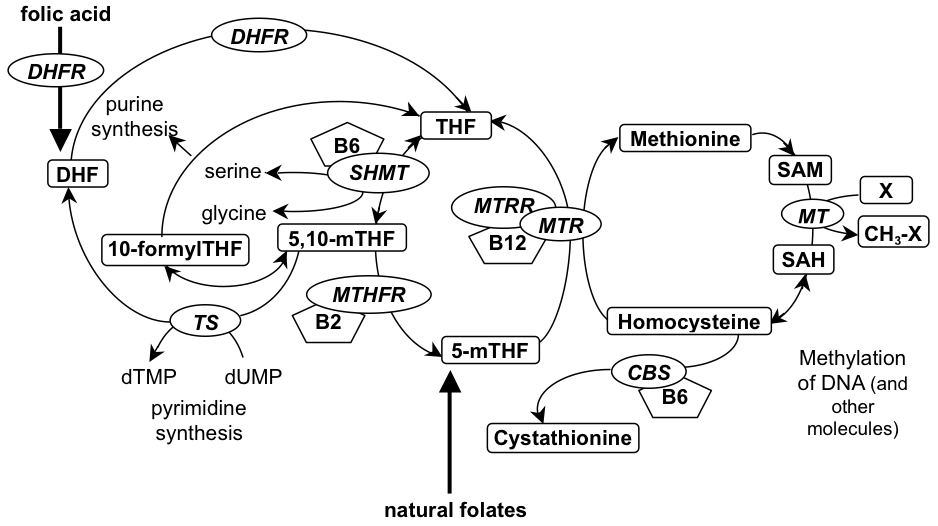
\includegraphics[width=0.85\textwidth]{ocm_xls5.jpg} 
\caption{Folate-mediated one-carbon metabolism. Abbreviations: DHF: dihydrofolate; DHFR: dihydrofolate reductase; THF: tetrahydrofolate; SHMT: serine hydroxymethyltransferase; 10-formylTHF: 10-formyltetrahydrofolate; 5,10-mTHF: 5,10-methylenetetrahydrofolate; 5-mTHF: 5-methyltetrahydrofolate; MTHFR: methylenetetrahydrofolate reductase; MTRR: methionine synthase reductase; MTR: methionine synthase; CBS: cystathionine $\beta$-synthase; MT: methyltransferase; SAM: \emph{S}-adenosylmethionine; SAH: \emph{S}-adenosylhomocysteine} 
\label{figure2_2} 
\end{figure}

\noindent Many enzymes are involved in folate-mediated one-carbon metabolism, and many of these enzymes require cofactors, which are often B vitamins. In addition to others, cobalamin (vitamin B12) is a cofactor for methionine synthase, an enzyme that converts homocysteine to methionine. Functional polymorphisms in enzyme-encoding genes involved in folate-mediated one-carbon metabolism play an important role in this cycle. A plethora of polymorphisms exist, but the most extensively studied polymorphism is a C-to-T substitution in methylenetetrahydrofolate reductase (MTHFR) at nucleotide 677, which converts alanine to valine resulting in decreased \emph{in vivo} enzyme activity \cite{c228}. Genetic polymorphisms and their interactions with nutrition in cancer are beyond the scope of this chapter, and only \emph{MTHFR} C677T will be mentioned in relation to nutrition, cancer, and epigenetics. Many studies on folate and human cancer risk have been conducted. In the following section, we describe the most prominent findings from observational studies, intervention studies, and randomised controlled trials (RCTs).

\subsubsection{Observational studies} % level 3
\paragraph{Colon and rectum} % level 4
The inverse association between high dietary folate intake and risk of colorectal adenomas was first seen and described both for women in the Nurses' Health Study and for men in the Health Professionals Follow-up Study \cite{c229}. Colorectal carcinomas often follow the adenoma-carcinoma sequence and adenomas are often used as a proxy endpoint for carcinomas \cite{c230}. The Nurses' Health Study is a cohort study that was initiated in 1976 to identify factors that influence women's health. Almost 122,000 US registered nurses, 30-55 years of age, completed a mailed questionnaire on risk factors for cancer and coronary heart disease, and 4 years later, they completed a semiquantitative food frequency questionnaire to assess diet from the previous year \cite{c231}. Similarly, the Health Professionals Follow-up Study began in 1986, and followed over 51,500 men, 40-75 years of age, who were dentists, optometrists, osteopaths, podiatrists, pharmacists, or veterinarians, to prospectively investigate dietary factors influencing cardiovascular disease and cancer risk. The men completed a semi-quantitative food frequency questionnaire designed to estimate average consumption during the past year \cite{c229,c232} found an inverse association between folate intake (from diet and supplements) and left colon and rectum adenoma risk (highest intake versus lowest intake multivariate relative risk (RR) = 0.71, 95\% confidence interval (CI) = 0.56-0.89). Those in the highest quintile of folate intake compared to those in the lowest quintile had a reduced risk of adenoma and this was true for both women (RR = 0.66, 95\%CI = 0.46-0.95) and men (RR = 0.63, 95\% CI = 0.41-0.98). There was a weak inverse association between folate intake from foods alone (supplement use excluded) and adenoma risk in women (RR = 0.91, 95\% CI=0.64-1.28) and men (RR = 0.78, 95\% CI = 0.52-1.17), again comparing those in the highest quintile of intake with the lowest. The association between alcohol intake and adenoma risk was also assessed, as alcohol 
is a well-known folate antagonist. Compared with nondrinkers, those who had more than 30 g of alcohol daily had a slightly (not significant) elevated risk of adenoma (RR=1.78, 95\% CI=1.28-2.47). Adenoma risk was highest for a combination high alcohol intake and low folate intake relative to a combination low alcohol intake and high folate intake (RR = 2.35, 95\% CI = 1.56-3.50). The multiple logistic regressions performed were adjusted for age, sex, body blood, occult fecal blood, abdominal pain, diarrhea (or constipation), and history of endoscopy prior to the study period. 
 
\noindent Results from a meta-analysis of seven cohort studies and nine case-control studies investigating the association between folate intake and CRC risk further demonstrated an inverse association between folate intake and CRC risk \cite{c233}. In the cohort studies a statistically significant reduced risk for CRC was observed in those with high dietary folate intake compared with those with low dietary folate intake (RR = 0.75, 95\% CI = 0.64-0.89), with no significant heterogeneity between studies. There was a nonsignificant inverse association between total folate intake and CRC risk (RR = 0.95, 95\% CI = 0.81-1.11), with no significant heterogeneity between studies. For case-control studies, a statistically significant decreased risk for CRC was also observed (for high vs. low intake RR=0.76, 95\%CI=0.60-0.96, although in this case there was evidence of heterogeneity between studies. There was a non-significant association between total folate intake and colorectal cancer (RR=0.81, 95\% CI=0.62-1.05), with no heterogeneity between studies. The meta-analyses included in the WCRF/AICR Second Expert Report used four cohort studies to elucidate the association between dietary folate intake and CRC. They reported a summary estimate of 0.84 (95\% CI=0.76-0.93) per 100 $\mu$g dietary folate per day, with no significant heterogeneity between studies \cite{c214}. 

\vspace{-0.4cm}
\paragraph{Pancreas} % level 4
A meta-analysis of three cohort studies analysing the link between folate intake and pancreatic cancer reported a protective effect of folate intake (summary cancer risk estimate 0.94, 95\% CI = 0.80-1.11) per 100 $\mu$g folate per day, with high heterogeneity between studies \cite{c214}. However, a recent cohort study did not find protective effects of folate and pancreatic cancer risk when comparing those in the highest folate intake quintile with those in the lowest folate intake quintile (adjusted hazard ratio (HR) = 1.37, 95\% CI = 0.97-1.94) \cite{c234}.

\vspace{-0.4cm}
\paragraph{Esophagus} % level 4 
The relationship between dietary folate and esophageal cancer risk has been explored only in observational case-control studies. Results from these studies indicated a decreased risk of esophageal cancer for those with the highest intake compared with those with the lowest intake \cite{c214}.

\vspace{-0.4cm}
\paragraph{Breast} % level 4
A meta-analysis has been carried out on the relationship between folate intake and risk of breast cancer. For prospective studies, there was no association between breast cancer for the highest \emph{versus} the lowest category of dietary folate intake (summary estimate = 0.96, 95\% CI = 0.87-1.05), with some heterogeneity. For case-control studies, there was a statistically significant inverse association between dietary folate intake and breast cancer risk (high \emph{versus} low intake summary estimate = 0.73, 95\% CI = 0.64-0.83), with no significant heterogeneity between studies \cite{c235}. 

\vspace{-0.4cm}
\paragraph{Prostate} % level 4 
Data on folate intake and prostate cancer risk are limited. A nested case-control study from Sweden reported a statistically significant positive association between plasma folate and prostate cancer risk (for highest \emph{versus} lowest quartile, odds ratio (OR) = 1.60, 95\% CI = 1.03-2.49). The risk for prostate cancer associated with B12 status was even stronger (highest \emph{versus} lowest quartile OR=2.63, 95\% CI=1.61-4.29) \cite{c236}. The European Prospective Investigation into Cancer and Nutrition (EPIC) Study group carried out an investigation of blood folate and vitamin B12 levels and prostate cancer risk. There was no significant association between blood folate and prostate cancer risk (highest intake quintile \emph{versus} lowest intake quintile adjusted RR = 1.30, 95\% CI = 0.88-1.93). Neither was there any association between vitamin B12 status and prostate cancer risk (Q5 \emph{versus} Q1 adjusted RR = 1.19, 95\% CI = 0.87-1.63) \cite{c237}. 
 
\subsubsection{Intervention studies} % level 3 
\noindent Potential protective effects of folic acid against several types of cancer have been explored using RCTs. 

\vspace{-0.4cm}
\paragraph{Colorectal cancer} % level 4 
The Aspirin/Folate Polyp Prevention Trial was a double-blind, placebo-controlled, randomised trial designed to study the efficacy of aspirin, folic acid, or both for colorectal adenoma recurrence in those with a history of adenomas. Participants were recruited at eight clinical centers in the United States and one in Canada over a period of approximately 4 years. Following a 3 x 2 factorial design, 1021 patients were randomised to receive either folic acid with or without aspirin or placebo with or without aspirin over a 3-year treatment period. Patients were invited to continue the trial for an additional 3 or 5 years if they had a colonoscopy within the first follow-up interval of 3 years. After the initial 3 years, the risk of developing at least one adenoma was 44.1\% for folic acid and 42.4\% for placebo (unadjusted RR = 1.04, 95\% CI = 0.90-1.20, P = 0.58). For those 607 who had a second follow-up, the risk of developing at least one adenoma was 41.9\% for folic acid and 37.2\% for placebo (unadjusted RR = 1.13, 95\% CI = 0.93-1.37, P = 0.23). Additionally, the risk of developing at least three adenomas after the second follow-up interval was 9.9\% for folic acid and 4.3\% for placebo (unadjusted RR = 2.32, 95\% CI = 1.23-4.35). Results from the Aspirin/Folate Polyp Prevention Trial, therefore, do not support the hypothesis that folic acid supplementation at 1 mg per day reduces colorectal adenoma risk in those with a history of adenomas \cite{c238}. 
 
\noindent A similar, but smaller, RCT -- the United Kingdom Colorectal Adenoma Prevention (UKCAP) Trial -- was carried out across nine centres in the United Kingdom and one in Denmark to study whether 300 mg aspirin per day or 0.5 mg folic acid supplementation per day in colorectal adenoma patients could prevent risk of colorectal adenoma recurrence over 3 years. Following a 2 x 2 factorial design, patients were randomised to receive either 300 mg aspirin or 0.5 mg folic acid or both or placebo for 3 years. The UKCAP study reported that the risk of recurrence of at least one adenoma was 26.6\% for those taking folic acid and 24.9\% for those taking placebo (RR = 1.07, 95\% CI = 0.85-1.34). Furthermore, the risk of developing at least one advanced adenoma was 12\% for those taking folic acid and 12.4\% for those taking placebo (RR = 0.98, 95\% CI = 0.68-1.40). There was no evidence that 0.5 mg folic acid supplementation reduced risk of colorectal adenoma recurrence \cite{c239}. Indeed, both studies report, if anything, an increased risk at these relatively high doses of folic acid though this effect was not significant in the smaller UKCAP trial and only significant for some measures in the larger Asprin/Folate Polyp trial. 
 
\noindent Animal studies have demonstrated that the protective effects of folate may depend on the time that it is given and that supplementation with folic acid may accelerate the progression of existing colorectal neoplasms \cite{c240,c241}. Whether or not this is also the case in humans requires further clarification. 

\vspace{-0.4cm}
\paragraph{Breast} % level 4 
The Women's Antioxidant and Folic Acid Cardiovascular Study, conducted in the United States, included 5442 female health professionals with pre-existing cardiovascular disease. These women, who had no cancer history, were randomised to receive either combined 2.5 mg folic acid per day, 50 mg vitamin B6 per day, and 1 mg vitamin B12 per day or placebo for 7.3 years in order to study the effect of combined folate, vitamin B6 (pyridoxine hydrochloride), and vitamin B12 on total invasive cancer or breast cancer prevention. There was no significant effect of treatment on risk of total invasive cancer (HR=0.97, 95\% CI=0.79-1.18; P = 0.75). Individual invasive cancers included were breast, colon and rectum, lung, uterine, ovary, lymphoma, leukemia, multiple myeloma, pancreas, kidney, urinary bladder, thyroid, skin melanoma, and others. For breast cancer, the HR was 0.83, 95\% CI = 0.60-1.14, P = 0.24. Combined supplementation with folic acid, vitamin B6, and vitamin B12 did not offer any significant effect on total invasive cancer or breast cancer risk among women \cite{c242}. 

\vspace{-0.4cm}
\paragraph{Prostate} % level 4 
Secondary analyses of the Aspirin/Folate Polyp Prevention Trial (see above) were performed to better understand the relationship between folic acid supplementation and prostate cancer risk. Six hundred forty-three men in the Aspirin/Folate Polyp Prevention Trial were randomised to receive either folic acid supplementation or placebo. Participants completed a semi-quantitative food frequency questionnaire, and non-fasting blood samples to measure the status of folate and other B vitamins were taken at the start of the trial. Baseline dietary folate intake (modelled as a continuous variable) was non-significantly inversely associated with prostate cancer risk (multi-variable adjusted HR = 0.65, 95\% CI = 0.35-1.20). Folic acid supplementation, on the other hand, was associated with a significantly increased risk of prostate cancer (multi-variable adjusted HR = 2.58, 95\% CI = 1.14-5.86) \cite{c243}. 
 
\noindent While abundant data on nutrition and cancer risk exist, these data are not always consistent and in many cases a clear picture in relation to individual nutrients has yet to emerge. 
 
\section[]{Nutrition and epigenetics} % level 1 
\noindent One way in which nutrition may modulate carcinogenesis is through epigenetic pathways. In human studies, the best demonstration for this are the ways in which folic acid affects DNA methylation in CRC. 
 
\subsection{Diet and DNA methylation patterns in observational studies} % level 2 
\noindent Two studies (one cohort study and one case-control study) reported an inverse association between dietary folate intake and promoter methylation in genes implicated in cancer -- \emph{APC-1A}, \emph{p14ARF}, \emph{p16INK4A}, \emph{hMLH1}, \emph{O6-MGMT}, and \emph{RASSF1A} -- and in carcinoma and adenoma tissue \cite{c211,c235}. In both studies, the relationship between folate intake and promoter methylation in genes implicated in CRC were investigated; the case-control study also included a subanalysis of the effect of \emph{MTHFR} C677T genotype on this relationship \cite{c219}. Those with a high dietary folate intake (>212 $\mu$g per day) were at decreased risk for having at least three genes methylated (OR for $\geq$3 methylated versus <3 methylated = 0.66, 95\% CI = 0.29--1.54), although this association was not statistically significant. In the cohort study, CRC patients were divided into two groups -- low folate/high alcohol and high folate/low alcohol. Those in the low folate/high alcohol intake group were at higher risk of having at least one gene methylated (84\%) compared with those in the high folate/low alcohol group (70\%, P = 0.085), though, again, this association was not statistically significant \cite{c244}. Subsequent follow-up of associations between dietary folate, vitamin B2, vitamin B6, methionine, and alcohol and \emph{MLH1} promoter methylation in the same cohort was carried out. Dietary folate intake did not affect \emph{MLH1} hypermethylation in men (tertile 3 \emph{versus} tertile 1 RR = 0.88, 95\% CI = 0.36-2.14) or women (tertile 3 \emph{versus} tertile 1 RR = 0.88, 95\% CI = 0.33-2.32). While there were no associations between folate intake and \emph{MLH1} hypermethylation, there was a significant positive association between vitamin B6 intake and \emph{MLH1} hypermethylation in men (high \emph{versus} low intake RR = 3.23, 95\% CI = 1.15-9.06) \cite{c245}. 
 
\noindent A case-control study investigated the risk of genomic DNA hypomethylation in response to folate status in colorectal adenoma patients and controls. DNA methylation patterns were determined in both leukocytes and adenoma tissues. Compared with controls, cancer patients had 26\% lower folate status (95\% CI = 6-44\%, P = 0.01). Adenoma tissue was 26\% (95\% CI = 8-56\%, P = 0.009) more hypomethylated than control tissues, while leukocyte DNA from those with adenomas was 16\% more (95\% CI = 8-30\%) hypomethylated than from those without adenomas \cite{c246}. 
 
\subsection{Diet and DNA methylation in intervention studies} % level 2 
\noindent Few studies have evaluated the relationship between controlled folate intake and global DNA methylation in humans. In the studies, healthy volunteers were fed low-folate diets followed by folate repletion and monitoring of global methylation in leukocytes. In one study, eight women were kept on a low-folate diet (56 $\mu$g folate per day to 516 $\mu$g folate per day) for 91 days in a metabolic ward. Blood was drawn on 13 occasions throughout the study period. Dietary folate was inversely associated with global DNA hypomethylation (analysis of variance (ANOVA) P < 0.001). Reversal of genome-wide DNA hypomethylation was observed following folate repletion at 286-516 $\mu$g folate per day \cite{c247}. A study of genomic DNA methylation in 33 elderly women showed similar results after folate depletion. These women were given a folate-deficient diet (118 $\mu$g folate per day) for 7 weeks followed by a folate-repletion diet of 200 or 415 $\mu$g folate per day for another 7 weeks. Global DNA hypomethylation in leukocytes was inversely related to folate intake (P = 0.0025), and this association was significant, but there were no significant changes to DNA methylation after folate repletion \cite{c248}. Two other folate depletion-repletion studies also looked into the effect of the \emph{MTHFR} C677T genotype on global leukocyte DNA methylation \cite{c249,c250}. Null associations were found between global leukocyte DNA methylation and folate depletion or repletion, and this association was not modified by \emph{MTHFR} C677T genotype (P > 0.05) for one study \cite{c240}, while the second study found a slight increase in global DNA methylation during folate repletion for those with the \emph{MTHFR} 677TT genotype \cite{c250}. 
 
\subsection{Folic acid, vitamin B12, and DNA methylation in randomised, placebo-controlled intervention trials} % level 2 
\noindent Randomised, placebo-controlled intervention trials in humans studying the relationship between nutrients and DNA methylation have, to date, been limited to folate and vitamin B12 supplementation. 
 
\subsubsection{Global DNA methylation} % level 3 
\noindent To our knowledge, eight randomised, placebo-controlled intervention trials investigating the effects of supplementation on DNA methylation have been published, nearly all of which have been carried out in patients with colorectal adenomas. Table 2.1 summarises these RCTs. Nearly all the studies used supraphysiological doses of folic acid. Two studies used volunteers without a past or present history of cancer \cite{c251,c252}. In a double-blinded, randomised, placebo-controlled, prospective trial conducted in Australia, 63 volunteers were recruited and given 2 mg folic acid per day and 20 $\mu$g vitamin B12 per day or a placebo for 12 weeks. Blood samples from the volunteers were collected at three time points throughout the intervention trial (baseline, midpoint, end). There were statistically significant increases in serum vitamin B12 (P=0.004) and red blood cell folate (P < 0.0001) and a decrease in plasma homocysteine (P < 0.0001) for those in the intervention group at the end compared with at the start of the trial. When comparing the difference between the placebo group and the intervention group at midpoint and baseline, there were also statistically significant increases in serum vitamin B12 (P = 0.01), red blood cell folate (P = 0.0001), and plasma homocysteine (P = 0.0001). However, the highly significant changes in B vitamin status were not reflected in global DNA methylation in the intervention group at the end compared with the start of the trial, nor when comparing the placebo group with the intervention group both at midpoint and at the end of the study \cite{c252}. 
 
\noindent In a 2006 study by Basten \emph{et al}. \cite{c251}, 61 healthy volunteers with red cell folate concentrations between 200 and 650 nmol/L were randomised to receive either 1.2 mg folic acid or a placebo for 12 weeks. Whole blood was obtained from volunteers at the start of the study and again after the intervention at week 12. The intervention had no significant effect on DNA methylation. 
 
\noindent Five of the other intervention trials, conducted in colorectal adenoma patients, assessed global methylation \cite{c253,c254,c255,c256,c257}, while one intervention trial looked into DNA methylation in promoter regions of specific genes \cite{c258} in colorectal tumour tissue. In a study carried out by Cravo \emph{et al}. in 1994, nonsignificant changes in DNA methylation levels were observed after 6 months in those who received placebo, but for those taking very high-dose folic acid (10 mg per day), there was a significant attenuation of tumour DNA hypomethylation (P < 0.02). DNA hypomethylation was significantly higher in carcinomas than in adenomas (P < 0.05) \cite{c253}. In a long-term crossover intervention trial, 6 months supplementation with folic acid caused an increase in global DNA methylation in 7 of 20 patients with adenomas (P = 0.05). Placebo treatment following folic acid supplementation returned global DNA methylation levels to their original values. This decrease in DNA hypomethylation resulting from folic acid intervention was significant only for those presenting a single polyp as opposed to multiple polyps (P = 0.007) \cite{c254}. In another study, folic acid supplementation in colorectal adenoma patients for 1 year significantly decreased their DNA hypomethylation levels at both 6 months and 1 year after the start of the intervention (P = 0.001), whereas for patients in the control group, placebo administration was associated with a significant increase in genomic DNA methylation only at 1 year (P = 0.04). At 6 months, there was also significantly higher genomic DNA methylation in the treatment group compared with placebo group (P = 0.02), but paradoxically this difference disappeared at 1 year. The authors suggest that the unknown factors that caused an increase in genomic DNA methylation in the placebo group warranted further investigation \cite{c255}. 
 
\noindent Results from a more recent trial in adenoma patients suggest that folic acid supplementation significantly attenuated global DNA hypomethylation in leukocytes and colonic mucosa \cite{c256}. The latest investigation on the relationship between folate and other B vitamins and LINE-1 (long interspersed nucleotide element, a retrotransposon that makes up 15\% of the human genome) methylation as a proxy for global DNA methylation was conducted as part of the Aspirin/Folate Polyp Prevention Study (see above). Three hundred eighty-eight participants from the Aspirin/Folate Polyp Prevention Study who consented to having normal bowel mucosa biopsies approximately 3 years after baseline were included in the analyses. Those randomised to the folic acid supplementation arm had greater LINE-1 methylation levels (mean = 64.53\%, 95\% CI = 64.16-64.90) compared with those in the placebo group (mean = 64.21\%, 95\% CI = 63.83-64.58, although this difference was not statistically significant. Total folate intake, multivitamin use, and dietary intake of vitamins B2 and B6 at baseline were not associated with LINE-1 methylation at baseline \cite{c257}. 

\noindent The picture emerging from these seven trials remains unclear, with some studies demonstrating decreases in global DNA hypomethylation \cite{c254,c256} and other studies showing no change \cite{c251,c252,c257}. Further research is required to fully delineate the consequences of supplementation as a form of chemoprevention. Epigenetic changes that occur in cancer are complex, with some genes being hypermethylated and others hypomethylated; therefore measures of global methylation may be of limited value in elucidating nutrient-mediated epigenetic effects in cancer. 

\subsubsection{Gene-promoter methylation} % level 3 
\noindent While multiple randomised, placebo-controlled intervention trials on folic acid supplementation and global DNA methylation have been conducted, to our knowledge, there has only been one on folic acid supplementation and promoter methylation \cite{c258}. Eighty-six patients with a history of colorectal adenomas were randomly assigned to receive a high dose of 5 mg folic acid per day plus 1.25 mg vitamin B12 per day or placebo for 6 months. Six tumour suppressor and DNA repair genes were assessed for promoter methylation in DNA from rectal biopsies at baseline and after the intervention. Results suggested that promoter hypermethylation occurred more often in the folic acid and vitamin B12 supplementation group compared with the placebo group though the effect was only approaching statistical significance. If there is folate deficiency, SAM is depleted and any DNA hypomethylation that might result from this has been hypothesised to cause DNA instability. This study suggests that extremely high intakes of folic acid (>1 mg per day) and vitamin B12 may be positively associated with DNA promoter hypermethylation in rectal mucosal DNA, indicating an optimal balance between global DNA hypomethylation and promoter-specific DNA hypermethylation.

\section{Conclusion} % level 1 
\noindent Body fatness, smoking, and an unhealthy diet are well-established risk factors for cancer. A healthy diet and other lifestyle habits are recommended to reduce the risk of cancers. Specific nutrients have been shown to influence carcinogenesis, and one mechanistic route may operate via an effect on epigenetic processes. This relationship has been most often studied in relation to folate and DNA methylation in CRC. However, the results from these studies are not entirely homogeneous, and this may be due in part to differences in study designs including DNA methylation assays, and duration, dose, and timing of exposure to folate/folic acid, which also require further clarification. The links between diet, epigenetics, and cancer are complicated but the hope is that, ultimately, diet could be used to reverse epigenetic modifications that predispose to cancer.

\begin{sidewaystable}[h]
\footnotesize
\caption{Randomised, placebo-controlled intervention trials on the effects of supplementation on DNA methylation.} 
\label{table2_1} 
  \begin{adjustbox}{width=18cm}
%  \setlength\extrarowheight{19pt}
%  \renewcommand{\arraystretch}{2.0}
  \begin{tabular}{L{2cm}C{3cm}C{3cm}C{2cm}C{2cm}C{4cm}}
  \hline
 ~ & ~ & ~ & ~ & ~ & ~\\
  \bfseries Study & \bfseries Number of participants & \bfseries Dose & \bfseries Cancer site & \bfseries Duration & \bfseries Endpoint\\
 ~ & ~ & ~ & ~ & ~ & ~\\
  \hline
 ~ & ~ & ~ & ~ & ~ & ~\\
\parbox[t][1.3cm]{2cm}{\raggedright Cravo \textit{et al.} 1994 \cite{c253}} &
\parbox[t][1.3cm]{3cm}{\centering 22 patients with adenomas or carcinomas and 8 healthy controls} &
\parbox[t][1.3cm]{3cm}{\centering 10mg folic acid} &
\parbox[t][1.3cm]{2cm}{\centering Colorectum} &
\parbox[t][1.3cm]{2cm}{\centering 6 months} &
\parbox[t][1.3cm]{4cm}{\centering Global DNA methylation in colorectal tissues}\\
 % \hline 
\parbox[t][1.2cm]{2cm}{\raggedright Cravo \textit{et al.} 1998 \cite{c254}} &
\parbox[t][1.2cm]{3cm}{\centering 20 adenoma patients} &
\parbox[t][1.2cm]{3cm}{\centering 5mg folic acid} &
\parbox[t][1.2cm]{2cm}{\centering Colorectum} &
\parbox[t][1.2cm]{2cm}{\centering 6 months} &
\parbox[t][1.2cm]{4cm}{\centering Global methylation in colorectal tissues}\\
 % \hline 
\parbox[t][1.2cm]{2cm}{\raggedright Fenech \textit{et al.} 1998 \cite{c252}} &
\parbox[t][1.2cm]{3cm}{\centering 63 volunteers} &
\parbox[t][1.2cm]{3cm}{\centering 2mg folic acid and 20\textrm{${\mu}$}g vitamin B12} &
\parbox[t][1.2cm]{2cm}{\centering None} &
\parbox[t][1.2cm]{2cm}{\centering 12 weeks} &
\parbox[t][1.2cm]{4cm}{\centering Global DNA methylation in leucocytes}\\
  % \hline 
\parbox[t][1.2cm]{2cm}{\raggedright Kim \textit{et al.} 2001 \cite{c255}} &
\parbox[t][1.2cm]{3cm}{\centering 20 adenoma patients} &
\parbox[t][1.2cm]{3cm}{\centering 5mg folic acid} &
\parbox[t][1.2cm]{2cm}{\centering Colorectum} &
\parbox[t][1.2cm]{2cm}{\centering 1 year} &
\parbox[t][1.2cm]{4cm}{\centering Global DNA methylation in colorectal tissues}\\
 % \hline 
\parbox[t][1.2cm]{2cm}{\raggedright Pufulete \textit{et al.} 2005 \cite{c256}} &
\parbox[t][1.2cm]{3cm}{\centering 31 adenoma patients} &
\parbox[t][1.2cm]{3cm}{\centering 400\textrm{${\mu}$}g folic acid} &
\parbox[t][1.2cm]{2cm}{\centering Colorectum} &
\parbox[t][1.2cm]{2cm}{\centering 10 weeks} &
\parbox[t][1.2cm]{4cm}{\centering Global DNA methylation in leucocytes and colorectal tissues} \\
  %\hline 
\parbox[t][1.2cm]{2cm}{\raggedright Basten \textit{et al.} 2006 \cite{c251}} &
\parbox[t][1.2cm]{3cm}{\centering 61 healthy volunteers} &
\parbox[t][1.2cm]{3cm}{\centering 1.2mg folic acid} &
\parbox[t][1.2cm]{2cm}{\centering None} &
\parbox[t][1.2cm]{2cm}{\centering 12 weeks} &
\parbox[t][1.2cm]{4cm}{\centering Global DNA methylation in lymphocytes}\\
 % \hline 
\parbox[t][1.2cm]{2cm}{\raggedright van den Donk \textit{et al.} 2007 \cite{c258}} &
\parbox[t][1.2cm]{3cm}{\centering 86 patients with history of adenomas} &
\parbox[t][1.2cm]{3cm}{\centering 5mg folic acid and 1.25mg vitamin B12} &
\parbox[t][1.2cm]{2cm}{\centering Colorectum} &
\parbox[t][1.2cm]{2cm}{\centering 6 months} &
\parbox[t][1.2cm]{4cm}{\centering Gene-promoter methylation in colorectal tissues} \\
  %\hline 
\parbox[t][1.2cm]{2cm}{\raggedright Figueiredo \textit{et al}. 2009 \cite{c257}} &
\parbox[t][1.2cm]{3cm}{\centering 388 adenoma patients} &
\parbox[t][1.2cm]{3cm}{\centering 1mg folic acid} &
\parbox[t][1.2cm]{2cm}{\centering Colorectum} &
\parbox[t][1.2cm]{2cm}{\centering 3 years} &
\parbox[t][1.2cm]{4cm}{\centering Global DNA methylation in colorectal tissues}\\
 \hline
  \end{tabular}
  \end{adjustbox}
\end{sidewaystable}

\begin{thebibliography}{12} 
	\bibitem{c21}	Szyf M, Pakneshan P, Rabbani SA. DNA methylation and breast cancer. Biochemical pharmacology. 2004 Sep 15;68(6):1187-97. 
	\bibitem{c22}	Gaudet MM, Campan M, Figueroa JD, Yang XR, Lissowska J, Peplonska B, et al. DNA hypermethylation of ESR1 and PGR in breast cancer: pathologic and epidemiologic associations. Cancer Epidemiol Biomarkers Prev. 2009 Nov;18(11):3036-43. 
	\bibitem{c23}	Hernandez-Vargas H, Lambert MP, Le Calvez-Kelm F, Gouysse G, McKay-Chopin S, Tavtigian SV, et al. Hepatocellular carcinoma displays distinct DNA methylation signatures with potential as clinical predictors. PloS one. 2010;5(3):e9749. 
	\bibitem{c24}	Ramos EA, Camargo AA, Braun K, Slowik R, Cavalli IJ, Ribeiro EM, et al. Simultaneous CXCL12 and ESR1 CpG island hypermethylation correlates with poor prognosis in sporadic breast cancer. BMC cancer. 2010;10:23. 
	\bibitem{c25}	Widschwendter M, Jiang G, Woods C, Muller HM, Fiegl H, Goebel G, et al. DNA hypomethylation and ovarian cancer biology. Cancer research. 2004 Jul 1;64(13):4472-80. 
	\bibitem{c26}	Fahrner JA, Eguchi S, Herman JG, Baylin SB. Dependence of histone modifications and gene expression on DNA hypermethylation in cancer. Cancer research. 2002 Dec 15;62(24):7213-8. 
	\bibitem{c27}	Kondo Y, Shen L, Issa JP. Critical role of histone methylation in tumor suppressor gene silencing in colorectal cancer. Molecular and cellular biology. 2003 Jan;23(1):206-15. 
	\bibitem{c28}	Fraga MF, Ballestar E, Villar-Garea A, Boix-Chornet M, Espada J, Schotta G, et al. Loss of acetylation at Lys16 and trimethylation at Lys20 of histone H4 is a common hallmark of human cancer. Nature genetics. 2005 Apr;37(4):391-400. 
	\bibitem{c29}	Jackson K, Yu MC, Arakawa K, Fiala E, Youn B, Fiegl H, et al. DNA hypomethylation is prevalent even in low-grade breast cancers. Cancer biology \& therapy. 2004 Dec;3(12):1225-31. 
	\bibitem{c210}	Russo AL, Thiagalingam A, Pan H, Califano J, Cheng KH, Ponte JF, et al. Differential DNA hypermethylation of critical genes mediates the stage-specific tobacco smoke-induced neoplastic progression of lung cancer. Clin Cancer Res. 2005 Apr 1;11(7):2466-70. 
	\bibitem{c211}	Garfinkel MD, Ruden DM. Chromatin effects in nutrition, cancer, and obesity. Nutrition (Burbank, Los Angeles County, Calif. 2004 Jan;20(1):56-62. 
	\bibitem{c212}	Nkondjock A, Shatenstein B, Maisonneuve P, Ghadirian P. Specific fatty acids and human colorectal cancer: an overview. Cancer detection and prevention. 2003;27(1):55-66. 
	\bibitem{c213}	Roynette CE, Calder PC, Dupertuis YM, Pichard C. n-3 polyunsaturated fatty acids and colon cancer prevention. Clinical nutrition (Edinburgh, Scotland). 2004 Apr;23(2):139-51. 
	\bibitem{c214}	World Cancer Research Fund / American Institute for Cancer Research. Food, Nutrition, Physical Activity, and the Prevention of Cancer: a Global Perspective. Washington DC: AICR, 2007. 
	\bibitem{c215}	Feinberg AP, Vogelstein B. Hypomethylation distinguishes genes of some human cancers from their normal counterparts. Nature. 1983 Jan 6;301(5895):89-92. 
	\bibitem{c216}	Lim U, Flood A, Choi SW, Albanes D, Cross AJ, Schatzkin A, et al. Genomic methylation of leukocyte DNA in relation to colorectal adenoma among asymptomatic women. Gastroenterology. 2008 Jan;134(1):47-55. 
	\bibitem{c217}	Moore LE, Pfeiffer RM, Poscablo C, Real FX, Kogevinas M, Silverman D, et al. Genomic DNA hypomethylation as a biomarker for bladder cancer susceptibility in the Spanish Bladder Cancer Study: a case-control study. The lancet oncology. 2008 Apr;9(4):359-66. 
	\bibitem{c218}	Fearon ER, Vogelstein B. A genetic model for colorectal tumorigenesis. Cell. 1990 Jun 1;61(5):759-67. 
	\bibitem{c219}	van den Donk M, van Engeland M, Pellis L, Witteman BJ, Kok FJ, Keijer J, et al. Dietary folate intake in combination with MTHFR C677T genotype and promoter methylation of tumor suppressor and DNA repair genes in sporadic colorectal adenomas. Cancer Epidemiol Biomarkers Prev. 2007 Feb;16(2):327-33. 
	\bibitem{c220}	Feinberg AP, Gehrke CW, Kuo KC, Ehrlich M. Reduced genomic 5-methylcytosine content in human colonic neoplasia. Cancer research. 1988 Mar 1;48(5):1159-61. 
	\bibitem{c221}	Ogino S, Nosho K, Kirkner GJ, Kawasaki T, Chan AT, Schernhammer ES, et al. A cohort study of tumoral LINE-1 hypomethylation and prognosis in colon cancer. Journal of the National Cancer Institute. 2008 Dec 3;100(23):1734-8. 
	\bibitem{c222}	Wilson VL, Smith RA, Ma S, Cutler RG. Genomic 5-methyldeoxycytidine decreases with age. The Journal of biological chemistry. 1987 Jul 25;262(21):9948-51. 
	\bibitem{c223}	Fraga MF, Ballestar E, Paz MF, Ropero S, Setien F, Ballestar ML, et al. Epigenetic differences arise during the lifetime of monozygotic twins. Proceedings of the National Academy of Sciences of the United States of America. 2005 Jul 26;102(30):10604-9. 
	\bibitem{c224}	Zhang K, Dent SY. Histone modifying enzymes and cancer: going beyond histones. Journal of cellular biochemistry. 2005 Dec 15;96(6):1137-48. 
	\bibitem{c225}	Lin RJ, Nagy L, Inoue S, Shao W, Miller WH, Jr., Evans RM. Role of the histone deacetylase complex in acute promyelocytic leukaemia. Nature. 1998 Feb 19;391(6669):811-4. 
	\bibitem{c226}	Zhu P, Martin E, Mengwasser J, Schlag P, Janssen KP, Gottlicher M. Induction of HDAC2 expression upon loss of APC in colorectal tumorigenesis. Cancer cell. 2004 May;5(5):455-63. 
	\bibitem{c227}	Mason JB, Dickstein A, Jacques PF, Haggarty P, Selhub J, Dallal G, et al. A temporal association between folic acid fortification and an increase in colorectal cancer rates may be illuminating important biological principles: a hypothesis. Cancer Epidemiol Biomarkers Prev. 2007 Jul;16(7):1325-9. 
	\bibitem{c228}	Frosst P, Blom HJ, Milos R, Goyette P, Sheppard CA, Matthews RG, et al. A candidate genetic risk factor for vascular disease: a common mutation in methylenetetrahydrofolate reductase. Nature genetics. 1995 May;10(1):111-3. 
	\bibitem{c229}	Giovannucci E, Stampfer MJ, Colditz GA, Rimm EB, Trichopoulos D, Rosner BA, et al. Folate, methionine, and alcohol intake and risk of colorectal adenoma. Journal of the National Cancer Institute. 1993 Jun 2;85(11):875-84. 
	\bibitem{c230}	Leslie A, Carey FA, Pratt NR, Steele RJ. The colorectal adenoma-carcinoma sequence. The British journal of surgery. 2002 Jul;89(7):845-60. 
	\bibitem{c231}	Willett WC, Stampfer MJ, Colditz GA, Rosner BA, Hennekens CH, Speizer FE. Dietary fat and the risk of breast cancer. The New England journal of medicine. 1987 Jan 1;316(1):22-8. 
	\bibitem{c232}	Rimm EB, Giovannucci EL, Willett WC, Colditz GA, Ascherio A, Rosner B, et al. Prospective study of alcohol consumption and risk of coronary disease in men. Lancet. 1991 Aug 24;338(8765):464-8. 
	\bibitem{c233}	Sanjoaquin MA, Allen N, Couto E, Roddam AW, Key TJ. Folate intake and colorectal cancer risk: a meta-analytical approach. International journal of cancer. 2005 Feb 20;113(5):825-8. 
	\bibitem{c234}	Keszei AP, Verhage BA, Heinen MM, Goldbohm RA, van den Brandt PA. Dietary folate and folate vitamers and the risk of pancreatic cancer in the Netherlands cohort study. Cancer Epidemiol Biomarkers Prev. 2009 Jun;18(6):1785-91. 
	\bibitem{c235}	Larsson SC, Giovannucci E, Wolk A. Folate and risk of breast cancer: a meta-analysis. Journal of the National Cancer Institute. 2007 Jan 3;99(1):64-76. 
	\bibitem{c236}	Hultdin J, Van Guelpen B, Bergh A, Hallmans G, Stattin P. Plasma folate, vitamin B12, and homocysteine and prostate cancer risk: a prospective study. International journal of cancer. 2005 Feb 20;113(5):819-24. 
	\bibitem{c237}	Johansson M, Appleby PN, Allen NE, Travis RC, Roddam AW, Egevad L, et al. Circulating concentrations of folate and vitamin B12 in relation to prostate cancer risk: results from the European Prospective Investigation into Cancer and Nutrition study. Cancer Epidemiol Biomarkers Prev. 2008 Feb;17(2):279-85. 
	\bibitem{c238}	Cole BF, Baron JA, Sandler RS, Haile RW, Ahnen DJ, Bresalier RS, et al. Folic acid for the prevention of colorectal adenomas: a randomized clinical trial. Jama. 2007 Jun 6;297(21):2351-9. 
	\bibitem{c239}	Logan RF, Grainge MJ, Shepherd VC, Armitage NC, Muir KR. Aspirin and folic acid for the prevention of recurrent colorectal adenomas. Gastroenterology. 2008 Jan;134(1):29-38. 
	\bibitem{c240}	Song J, Medline A, Mason JB, Gallinger S, Kim YI. Effects of dietary folate on intestinal tumorigenesis in the apcMin mouse. Cancer research. 2000 Oct 1;60(19):5434-40. 
	\bibitem{c241}	Song J, Sohn KJ, Medline A, Ash C, Gallinger S, Kim YI. Chemopreventive effects of dietary folate on intestinal polyps in Apc+/-Msh2-/- mice. Cancer research. 2000 Jun 15;60(12):3191-9. 
	\bibitem{c242}	Zhang SM, Cook NR, Albert CM, Gaziano JM, Buring JE, Manson JE. Effect of combined folic acid, vitamin B6, and vitamin B12 on cancer risk in women: a randomized trial. Jama. 2008 Nov 5;300(17):2012-21. 
	\bibitem{c243}	Figueiredo JC, Grau MV, Haile RW, Sandler RS, Summers RW, Bresalier RS, et al. Folic acid and risk of prostate cancer: results from a randomized clinical trial. Journal of the National Cancer Institute. 2009 Mar 18;101(6):432-5. 
	\bibitem{c244}	van Engeland M, Weijenberg MP, Roemen GM, Brink M, de Bruine AP, Goldbohm RA, et al. Effects of dietary folate and alcohol intake on promoter methylation in sporadic colorectal cancer: the Netherlands cohort study on diet and cancer. Cancer research. 2003 Jun 15;63(12):3133-7. 
	\bibitem{c245}	de Vogel S, Bongaerts BW, Wouters KA, Kester AD, Schouten LJ, de Goeij AF, et al. Associations of dietary methyl donor intake with MLH1 promoter hypermethylation and related molecular phenotypes in sporadic colorectal cancer. Carcinogenesis. 2008 Sep;29(9):1765-73. 
	\bibitem{c246}	Pufulete M, Al-Ghnaniem R, Leather AJ, Appleby P, Gout S, Terry C, et al. Folate status, genomic DNA hypomethylation, and risk of colorectal adenoma and cancer: a case control study. Gastroenterology. 2003 May;124(5):1240-8. 
	\bibitem{c247}	Jacob RA, Gretz DM, Taylor PC, James SJ, Pogribny IP, Miller BJ, et al. Moderate folate depletion increases plasma homocysteine and decreases lymphocyte DNA methylation in postmenopausal women. The Journal of nutrition. 1998 Jul;128(7):1204-12. 
	\bibitem{c248}	Rampersaud GC, Kauwell GP, Hutson AD, Cerda JJ, Bailey LB. Genomic DNA methylation decreases in response to moderate folate depletion in elderly women. The American journal of clinical nutrition. 2000 Oct;72(4):998-1003. 
	\bibitem{c249}	Axume J, Smith SS, Pogribny IP, Moriarty DJ, Caudill MA. Global leukocyte DNA methylation is similar in African American and Caucasian women under conditions of controlled folate intake. Epigenetics. 2007 Jan-Mar;2(1):66-8. 
	\bibitem{c250}	Shelnutt KP, Kauwell GP, Gregory JF, 3rd, Maneval DR, Quinlivan EP, Theriaque DW, et al. Methylenetetrahydrofolate reductase 677C $\rightarrow$ T polymorphism affects DNA methylation in response to controlled folate intake in young women. The Journal of nutritional biochemistry. 2004 Sep;15(9):554-60. 
	\bibitem{c251}	Basten GP, Duthie SJ, Pirie L, Vaughan N, Hill MH, Powers HJ. Sensitivity of markers of DNA stability and DNA repair activity to folate supplementation in healthy volunteers. British journal of cancer. 2006 Jun 19;94(12):1942-7. 
	\bibitem{c252}	Fenech M, Aitken C, Rinaldi J. Folate, vitamin B12, homocysteine status and DNA damage in young Australian adults. Carcinogenesis. 1998 Jul;19(7):1163-71. 
	\bibitem{c253}	Cravo M, Fidalgo P, Pereira AD, Gouveia-Oliveira A, Chaves P, Selhub J, et al. DNA methylation as an intermediate biomarker in colorectal cancer: modulation by folic acid supplementation. Eur J Cancer Prev. 1994 Nov;3(6):473-9. 
	\bibitem{c254}	Cravo ML, Pinto AG, Chaves P, Cruz JA, Lage P, Nobre Leitao C, et al. Effect of folate supplementation on DNA methylation of rectal mucosa in patients with colonic adenomas: correlation with nutrient intake. Clinical nutrition (Edinburgh, Scotland). 1998 Apr;17(2):45-9. 
	\bibitem{c255}	Kim YI, Baik HW, Fawaz K, Knox T, Lee YM, Norton R, et al. Effects of folate supplementation on two provisional molecular markers of colon cancer: a prospective, randomized trial. The American journal of gastroenterology. 2001 Jan;96(1):184-95. 
	\bibitem{c256}	Pufulete M, Al-Ghnaniem R, Khushal A, Appleby P, Harris N, Gout S, et al. Effect of folic acid supplementation on genomic DNA methylation in patients with colorectal adenoma. Gut. 2005 May;54(5):648-53. 
	\bibitem{c257}	Figueiredo JC, Grau MV, Wallace K, Levine AJ, Shen L, Hamdan R, et al. Global DNA hypomethylation (LINE-1) in the normal colon and lifestyle characteristics and dietary and genetic factors. Cancer Epidemiol Biomarkers Prev. 2009 Apr;18(4):1041-9. 
	\bibitem{c258}	van den Donk M, Pellis L, Crott JW, van Engeland M, Friederich P, Nagengast FM, et al. Folic acid and vitamin B-12 supplementation does not favorably influence uracil incorporation and promoter methylation in rectal mucosa DNA of subjects with previous colorectal adenomas. The Journal of nutrition. 2007 Sep;137(9):2114-20. 
\end{thebibliography} 
